\title{Git Assistant}
\author{Ali AlShami}


%Main body starts
\section{Introduction}
I am Ali Alshami, a Ph.D. student in computer science and a Graduate Research Assistant (GRA) at the Vision Security Technology (VAST) Lab, the University of Colorado Colorado Springs (UCCS).

My goal for the course is to finish and submit a survey paper on human action recognition and prediction and start a new paper that focuses on predicting the future movement of humans based on human pose estimation and motion information. The survey paper reviews and evaluates the recent human actions recognition and prediction papers based on vision and machine learning. The new work will be focused on predicting the future movement of humans in video based on past movement, motion information, and human pose estimation.

I hope to learn more about improving my research skills and what I must consider becoming a better researcher. I am also curious about how to convert research that we are working on to a product you and what things we need to consider to make it a successful product.

I enjoy outdoor activities, including running, hiking, mountain biking, tennis, pickle-ball, and snowboarding. I also like reading and playing piano sometimes.
\begin{figure}[hbt!]
    \centering
    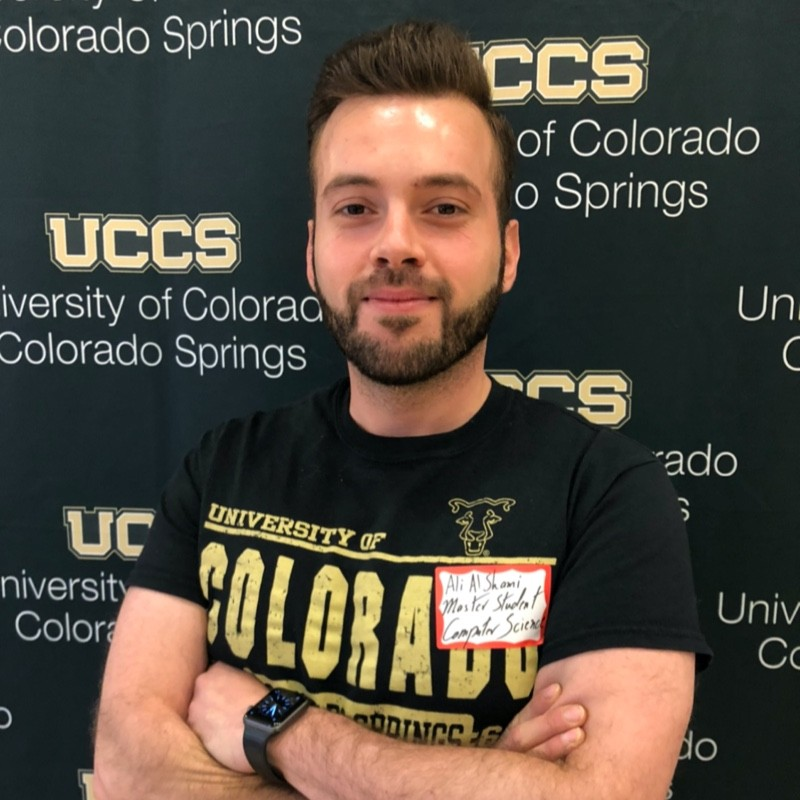
\includegraphics[width=5cm]{alshami.jpg}
    \caption{ }
    \label{fig:Remove}
\end{figure}

\section{Related code}
One of the new papers that I read now calld Multiview Transformer for video recognition.
The MTV model consists of separate encoders to represent different views of the input video with lateral connection to fuse information across views.
Chect the git repo here: https://github.com/google-research/scenic/tree/main/scenic/projects/mtv

\section{Ask question here}
Question from Noah:
If you dont mind me asking what was your masters and bachelors in because Im curious on what led to that specific topic of research? If its the same as your Ph.D. then what did lead to you becoming intrested in your area of research? -Noah Rodgers
I have a bachelor's degree in software engineering and a master's in computer science. I have started work on this topic before for my master's degree and now continue on the same path.
Question from Jose:
We coincide in the idea about making your research a product. Are you willing or have you considered patenting your research? - Jose Remy
Great question. Human action recognition has been applied in many applications, and I hope to patent my research in the future. 
\bibliographystyle{IEEEtran}
\bibliography{main}

\end{document}